\documentclass[10pt]{article}
\usepackage[ngerman]{babel}
\usepackage[utf8]{inputenc}
\usepackage[T1]{fontenc}
\usepackage{graphicx}
\usepackage[export]{adjustbox}
\graphicspath{ {./images/} }

\title{Bachelor of Science (BSc) in Informatik }

\author{SWEN1/PM3 Team:\\
R. Ferri (feit), D. Liebhart (lieh), K. Bleisch (bles), G. Wyder (wydg)}
\date{}


\begin{document}
\maketitle
\section*{Modul Software-Entwicklung 1 (SWEN1) }
\section*{LE 03 - Anforderungsanalyse II Zusammenfassung}


\section*{Warm-Up}
\begin{itemize}
  \item Wo stehen wir im Software-Entwicklungsprozess nach der Anforderungsanalyse I?
  \item Was sind die 3 wichtigsten Usability-Anforderungen?
  \item Welche Artefakte werden typischerweise im UCD erstellt und was beschreiben sie?
\end{itemize}

\section*{Um was geht es?}
\begin{itemize}
  \item Wie bringt man UCD in SWE-Prozesse ein?\\
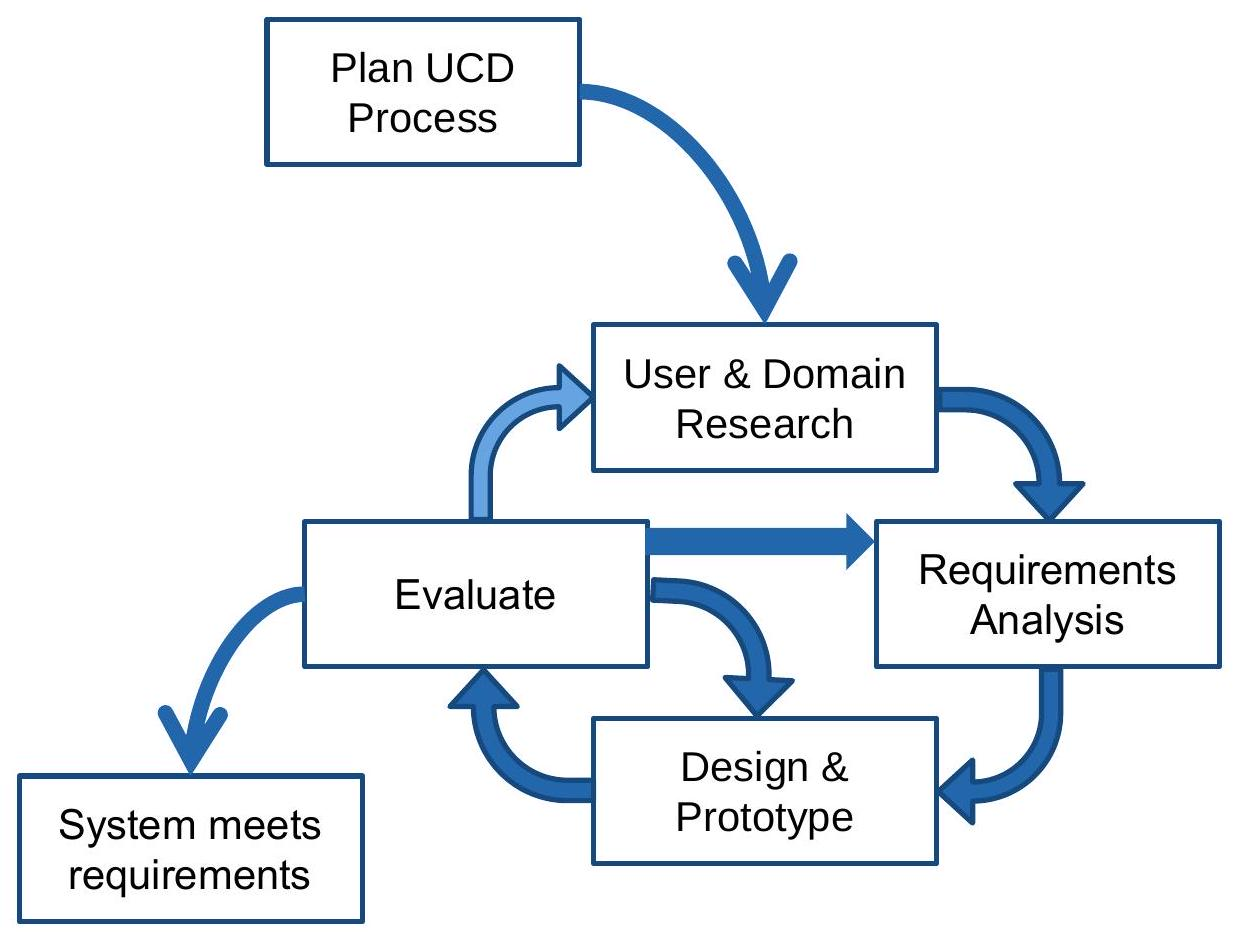
\includegraphics[width=\linewidth]{images/2025_01_02_6d70b14c9f1b57c2938fg-03}
\end{itemize}

UX-Team\\
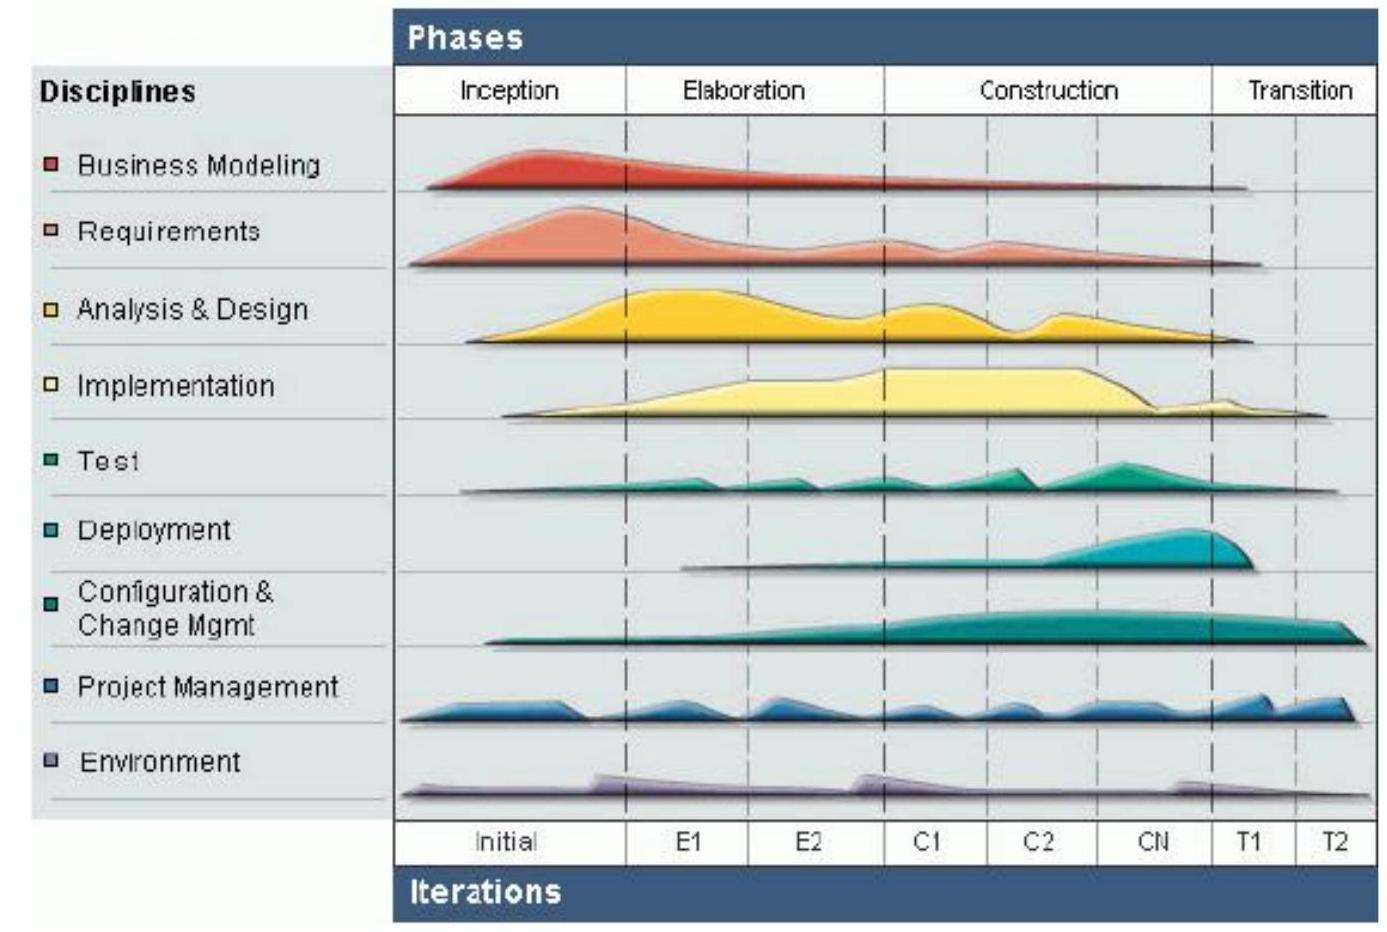
\includegraphics[width=\linewidth]{images/2025_01_02_6d70b14c9f1b57c2938fg-03(1)}

SWE-Team

\section*{Anforderungsanalyse: Benutzer-Anforderungen}
\begin{center}
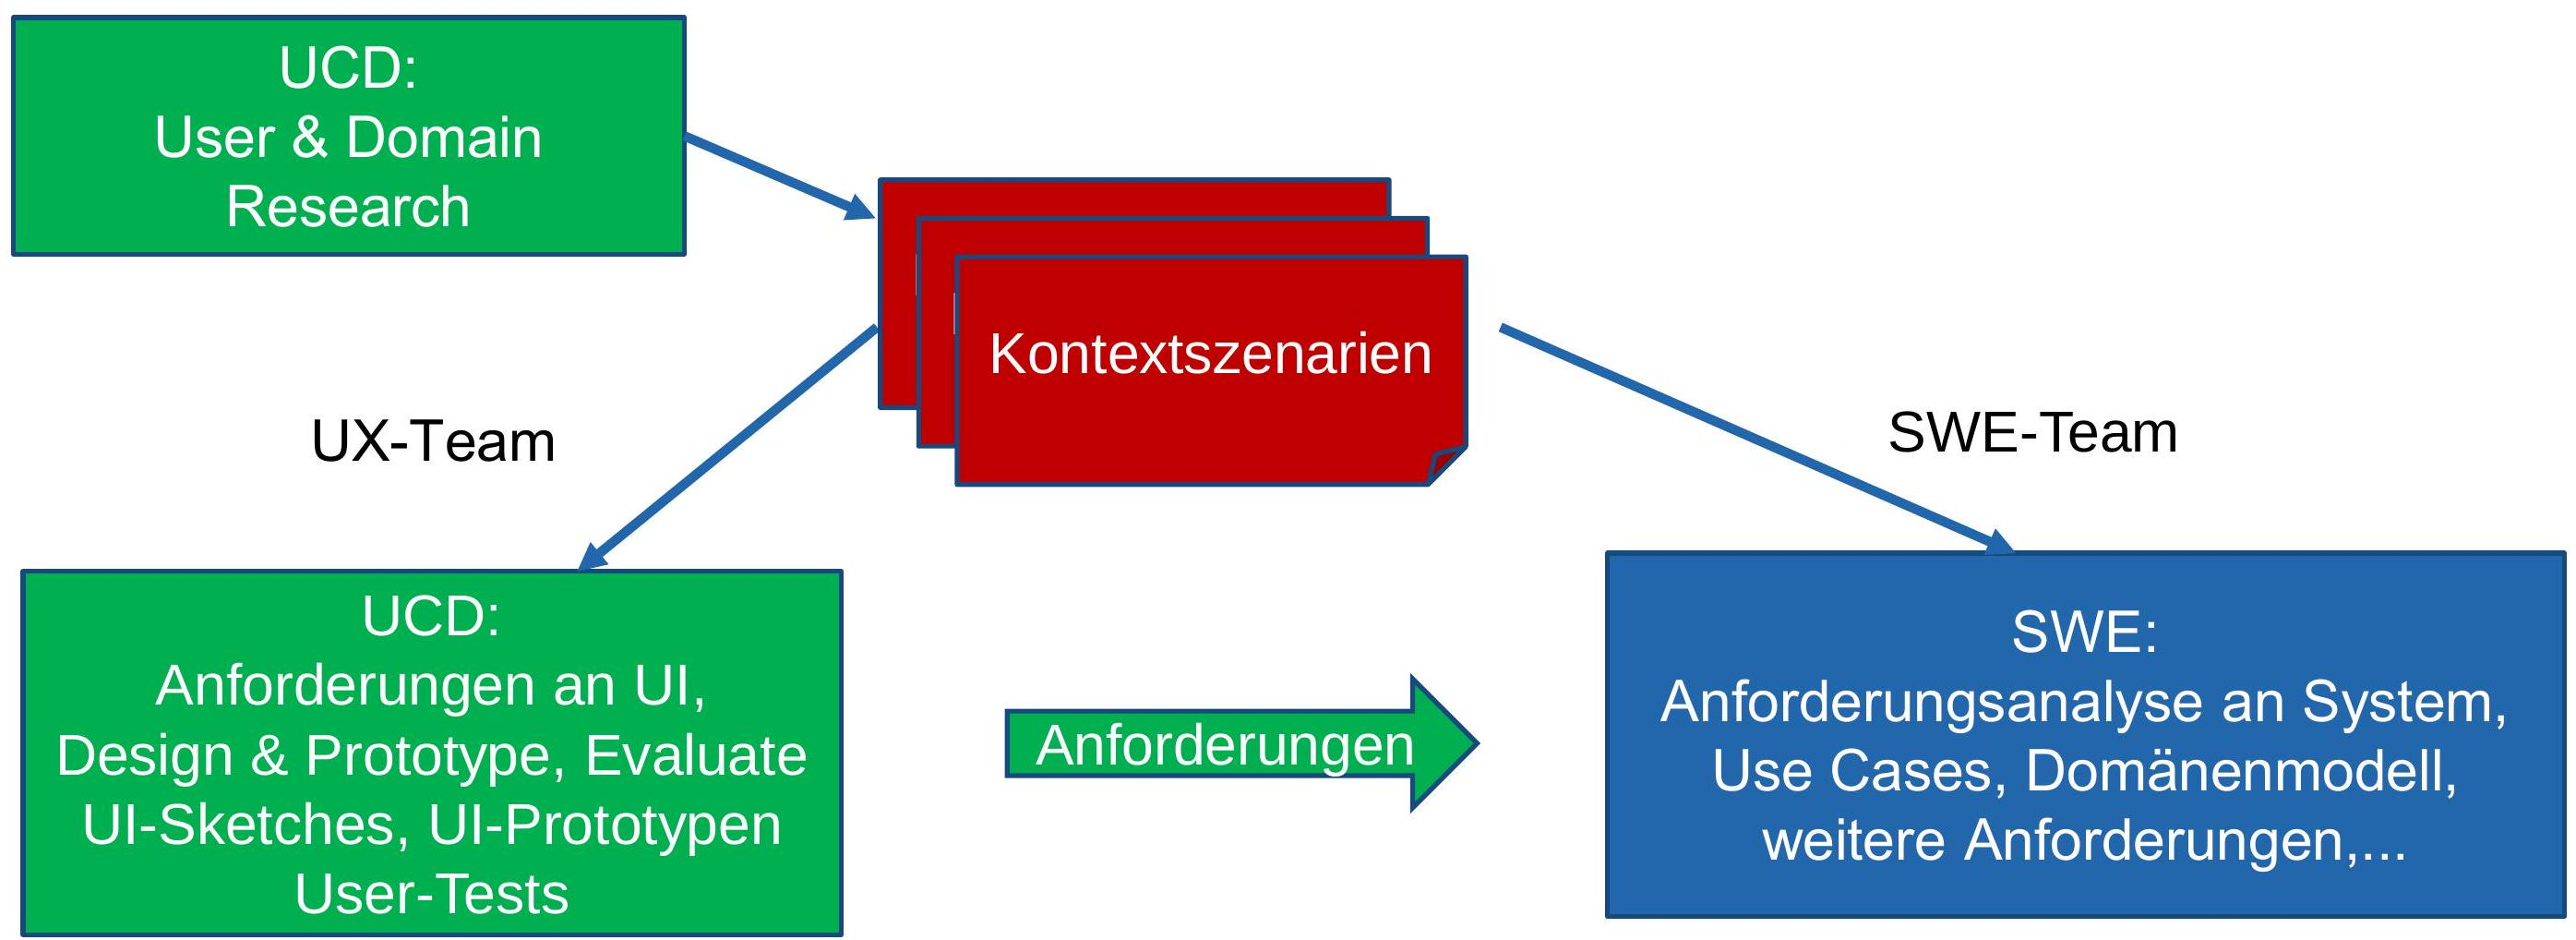
\includegraphics[width=\linewidth]{images/2025_01_02_6d70b14c9f1b57c2938fg-04}
\end{center}

\section*{Lernziele LE 03 - Anforderungsanalyse II}
Sie sind in der Lage,

\begin{itemize}
  \item aus den Artefakten des UCD detaillierte Anforderungen an das Softwareprodukt und dessen UI abzuleiten.
  \item funktionale Anforderungen in Form von Use Cases in verschiedenen Granularitätsstufen aus Kontextszenarien abzuleiten.
  \item weitere funktionale und nicht-funktionale Anforderungen aus den Artefakten des UCD abzuleiten.
\end{itemize}

\begin{enumerate}
  \item Wie erfasst man (dynamische) funktionale Anforderungen mit Use Cases
  \item Wie schreibt man gute Use Cases
  \item System-Sequenzdiagramme, Systemoperationen und Verträge
  \item Wie erfasst man zusätzliche funktionale und nicht-funktionale Anforderungen
  \item Wrap-up und Ausblick
\end{enumerate}

\section*{SWE: Anforderungsanalyse}
\begin{itemize}
  \item Anforderungen (Requirements)
  \item Forderungen bezüglich (Leistungs-) Fähigkeiten oder Eigenschaften, die das System/Projekt unter gegebenen Bedingungen erfüllen muss
  \item Können explizit oder implizit sein
  \item Kurze Diskussion
  \item Woher kommen die Anforderungen an ein System und wieso?
\end{itemize}

\begin{enumerate}
  \item Benutzer (möchte einen Job erledigen in einem bestimmten Kontext, hat bestimmte Bedürfnisse, Skills, Ziele)
  \item Weitere Stakeholder (Einkauf, Projektleiter, IT-Abteilung, ...)
  \item Regulatorien, Gesetze, Normen
\end{enumerate}

\section*{SWE: Anforderungsanalyse}
\begin{itemize}
  \item Anforderungen (Requirements)
  \item Sind (fast) nie im Vorneherein vollständig bekannt
  \item Müssen zusammen mit den Benutzern und anderen Stakeholdern erarbeitet werden
  \item Sie haben häufig implizite Anforderungen nicht explizite
  \item Explizite Anforderungen sollten hinterfragt werden (wieso bestehen sie genau so)
  \item Können kaum je zu Beginn vollständig erhoben werden, sondern entwickeln sich im Verlaufe des Projekts
  \item «I don't know what I want but I'll tell you when I see it!»
  \item Problematisch bei nicht iterativen Prozessen
\end{itemize}

\section*{Anforderungsanalyse: Anwendungsfälle (Use Cases)}
\begin{itemize}
  \item Textuelle Beschreibung einer konkreten Interaktion eines bestimmten Benutzers mit dem zukünftigen System
  \item Aus Sicht des Akteurs
  \item Enthalten implizite und explizite Anforderungen
  \item Beschreiben das Ziel des Benutzers (= Grund für die Anforderungen)
  \item Beschreiben den Kontext
\end{itemize}

\section*{Anforderungsanalyse: Anwendungsfälle (Use Cases)}
\begin{itemize}
  \item Use Cases (UCs) bilden in iterativen SWE-Prozessen eine zentrale Rolle
  \item Funktionale Anforderungen werden hauptsächlich mit UCs dokumentiert
  \item Mittels UCs können Anforderungen einfach mit dem Kunden diskutiert werden
  \item UCs sind ein wichtiger Teil der iterativen Projektplanung
  \item Projekt wird entlang von UCs geplant
  \item UC-Realisierungen bestimmen die Lösungsarchitektur und treiben das Lösungsdesign
  \item UCs werden für funktionale Systemtests eingesetzt
  \item UCs bilden die Basis für Benutzerhandbücher
\end{itemize}

\section*{Anforderungsanalyse: Anwendungsfälle (Use Cases)}
\begin{itemize}
  \item 3 Ausprägungen von Anwendungsfällen
  \item Kurz (Brief UC)
  \item Titel + 1 Absatz
  \item Beschreibt Standardablauf (keine Varianten, Problemfälle)
  \item Informell (Casual UC)
  \item Titel + informelle Beschreibung in ein bis mehrere Absätze
  \item Beschreibt auch wichtige Varianten
  \item Vollständig (Fully dressed UC)
  \item Titel + alle Schritte und Varianten werden im Detail beschrieben
  \item Enthalten weitere Informationen zu Vorbedingungen, Erfolgsgarantien, etc.
\end{itemize}

\section*{Anforderungsanalyse: Anwendungsfälle (Use Cases)}
\begin{itemize}
  \item Umfang eines guten Use Case
  \item Muss einen konkreten Nutzen für den Akteur erzeugen
  \item Eine Handlung, die eine Person, an einem Ort zu einer Zeit mit dem System ausführt
  \item Sollte mehr als eine einzelne Interaktion umfassen
  \item Titel eines UC
  \item Aktiv formulieren
  \item Verb! + evtl. Objekt vorangestellt (z.B. „Kasse eröffnen")
  \item Sollte Ziel des Akteurs beschreiben
  \item Boss-Test
  \item Falls dein Boss dich fragt, was du den ganzen Tag gemacht hast und du sagt, du hast die ganze Zeit den einen Use Case ausgeführt, sollte er zufrieden sein!
  \item EBP-Test (Elementary Business Proc.)
  \item Eine Aufgabe, die von einer Person an einem Ort zu einer bestimmten Zeit ausgeführt wird, als Reaktion auf einen Business Event.
  \item Size-Test
  \item Mehr als eine einzelne Interaktion
  \item Fully dressed meist mehrere Seiten lang
\end{itemize}

\section*{Finden von Anwendungsfällen}
\begin{itemize}
  \item Schritt 1: Systemgrenzen definieren
  \item Kasse
  \item Schritt 2: Primärakteure identifizieren
  \item Kassier
  \item Frage: Wieso nicht Kunde?\\

\includegraphics[width=\linewidth]{images/2025_01_02_6d70b14c9f1b57c2938fg-13}
\end{itemize}

Steuerbehörde\\

\includegraphics[width=\linewidth]{images/2025_01_02_6d70b14c9f1b57c2938fg-13(1)}

Kioskkunde\\
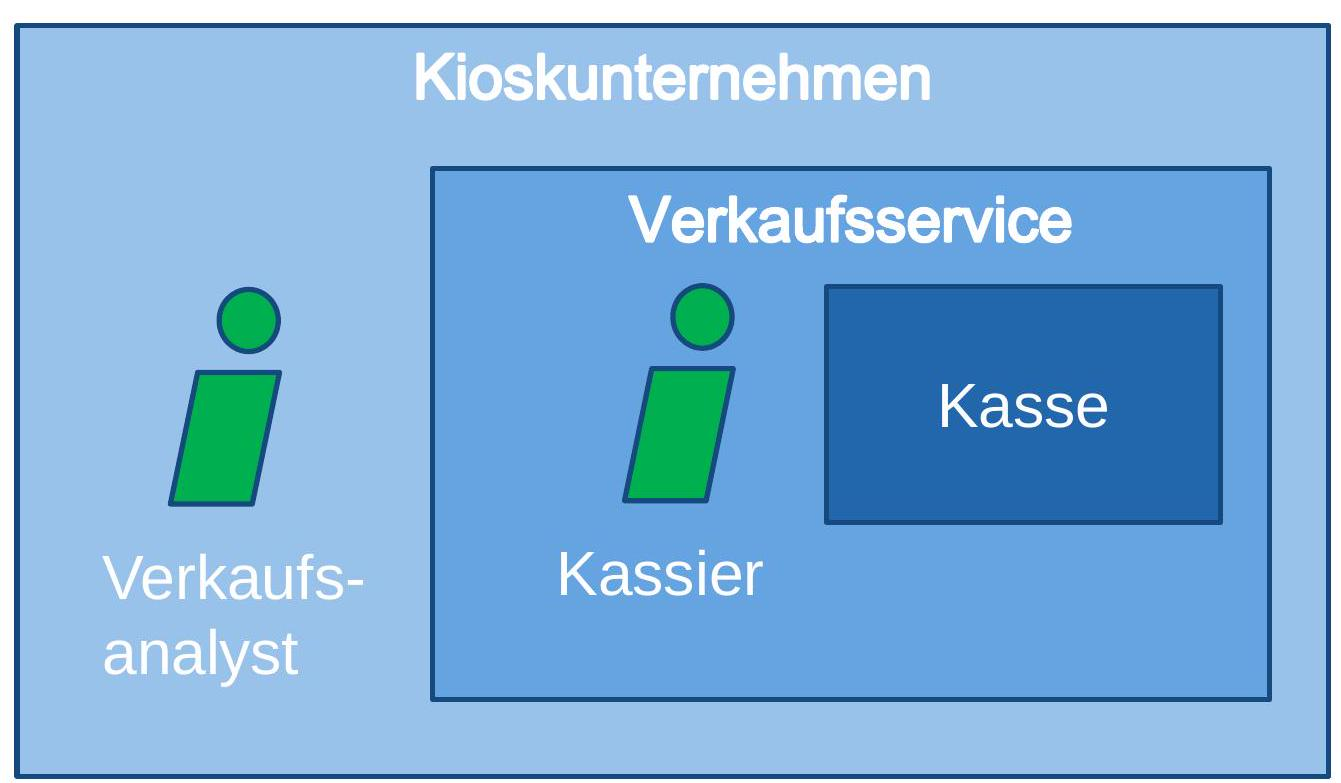
\includegraphics[width=\linewidth]{images/2025_01_02_6d70b14c9f1b57c2938fg-13(2)}

\section*{Finden von Anwendungsfällen}
\begin{itemize}
  \item Schritt 1: Systemgrenzen definieren
  \item Kasse
  \item Schritt 2: Primärakteure identifizieren
  \item Kassier
  \item Frage: Wieso nicht Kunde?
  \item Schritt 3:
  \item Jobs (Ziele, Aufgaben) der Primärakteure identifizieren
  \item Kassier
  \item Kasse eröffnen
  \item Verkauf abwickeln
  \item Kasse abrechnen
  \item Retouren entgegennehmen
  \item Kassenadministrator
  \item Kasse aufsetzen
  \item Kasse warten
  \item Kasse ausser Betrieb nehmen
  \item Kassenbenutzer administrieren
\end{itemize}

\section*{Anwendungsfalldiagramm (Use-Case-Diagramm)}
\begin{itemize}
  \item Zeigt
  \item Systemabgrenzung
  \item Akteure
  \item Primärakteure initiieren einen UC
  \item Unterstützende Akteure sind beteiligt an einem UC
  \item Liste der Anwendungsfälle
\end{itemize}

\begin{enumerate}
  \item Process Sale
  \item Cash In
  \item Cash Out
  \item Handle Returns
  \item Manage Users\\
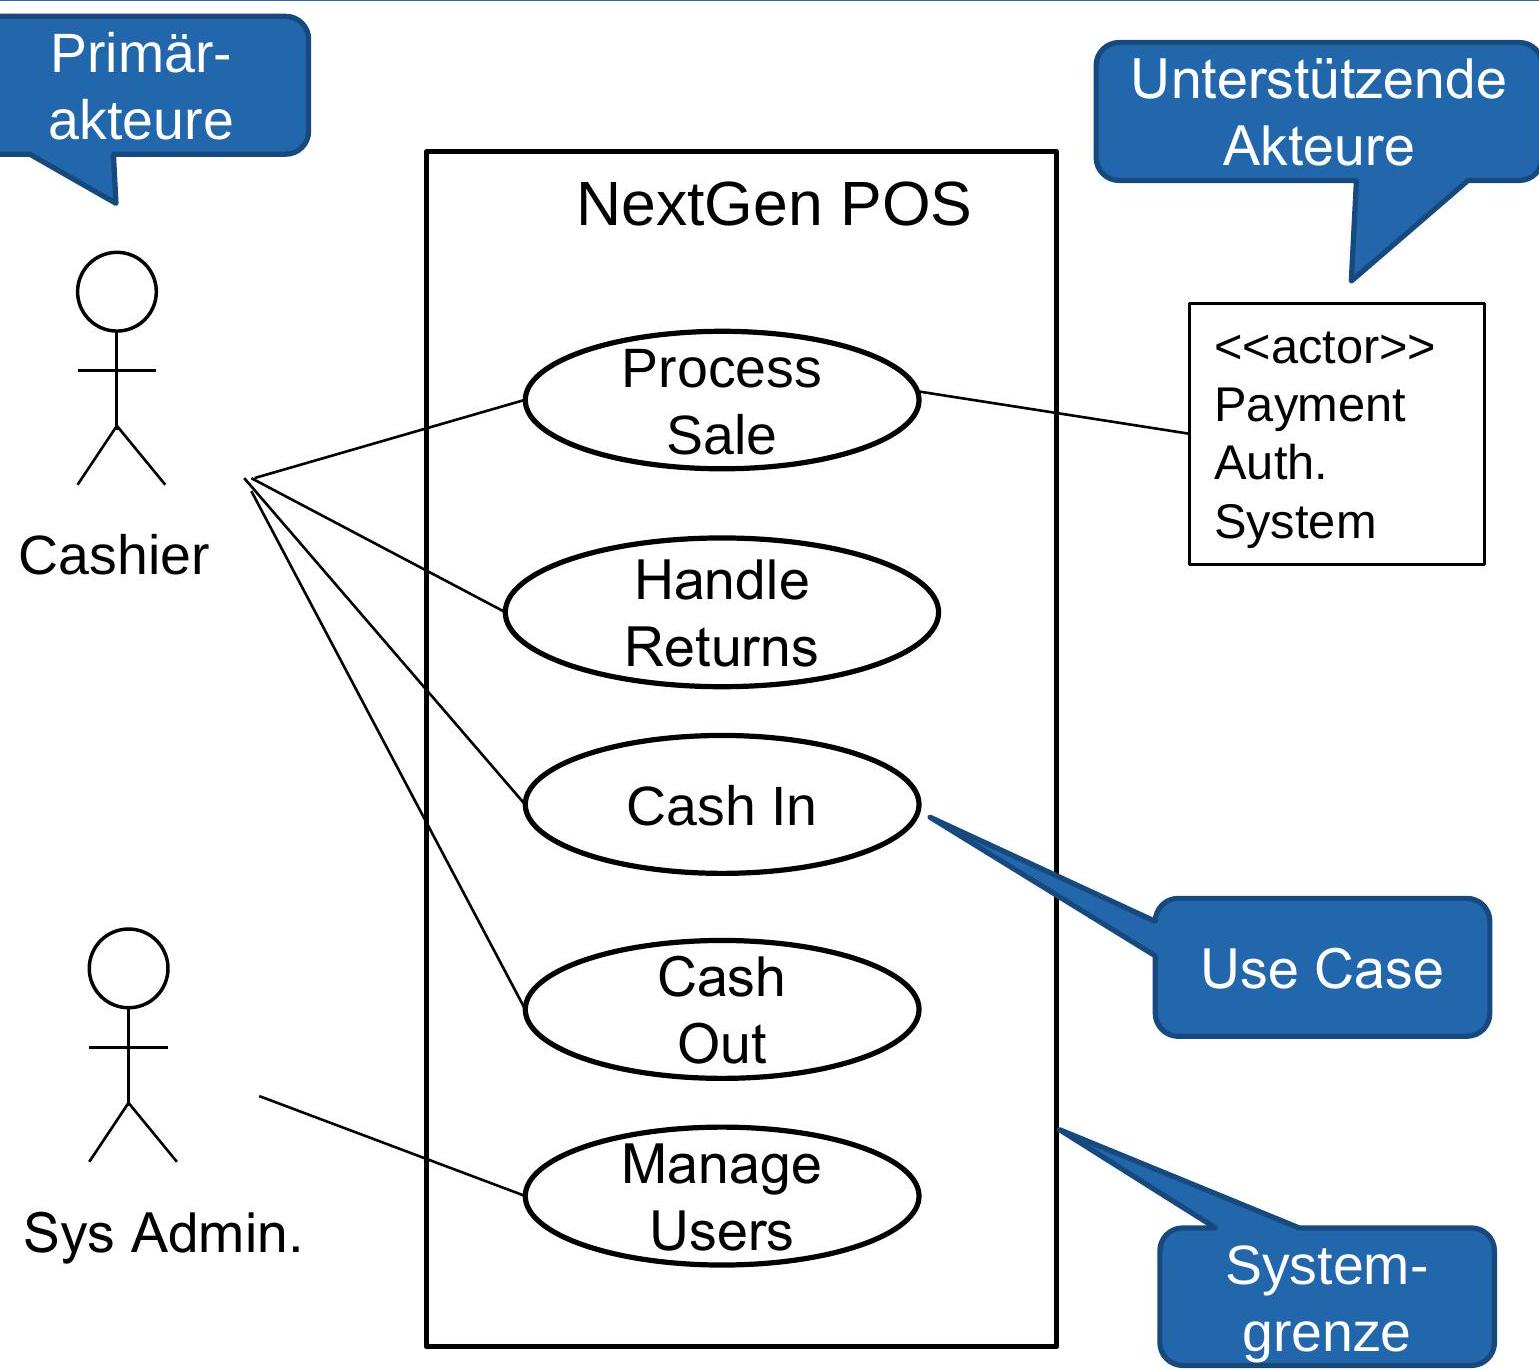
\includegraphics[width=\linewidth]{images/2025_01_02_6d70b14c9f1b57c2938fg-15}
\end{enumerate}

\section*{Anwendungsfalldiagramm (Use-Case-Diagramm)}
School of

\begin{itemize}
  \item Zusätzliche Beziehungen im UC-Diagramm
  \item <<include>>
  \item UC "Handle Cash Payment" und UC „Handle TWINT Payment" sind enthalten im UC „Process Sale"
  \item Sie sind hier aber keine eigenständigen UCs (keine Verbindung zu Akteuren)
  \item Included UCs können auch selbständige UC sein.\\
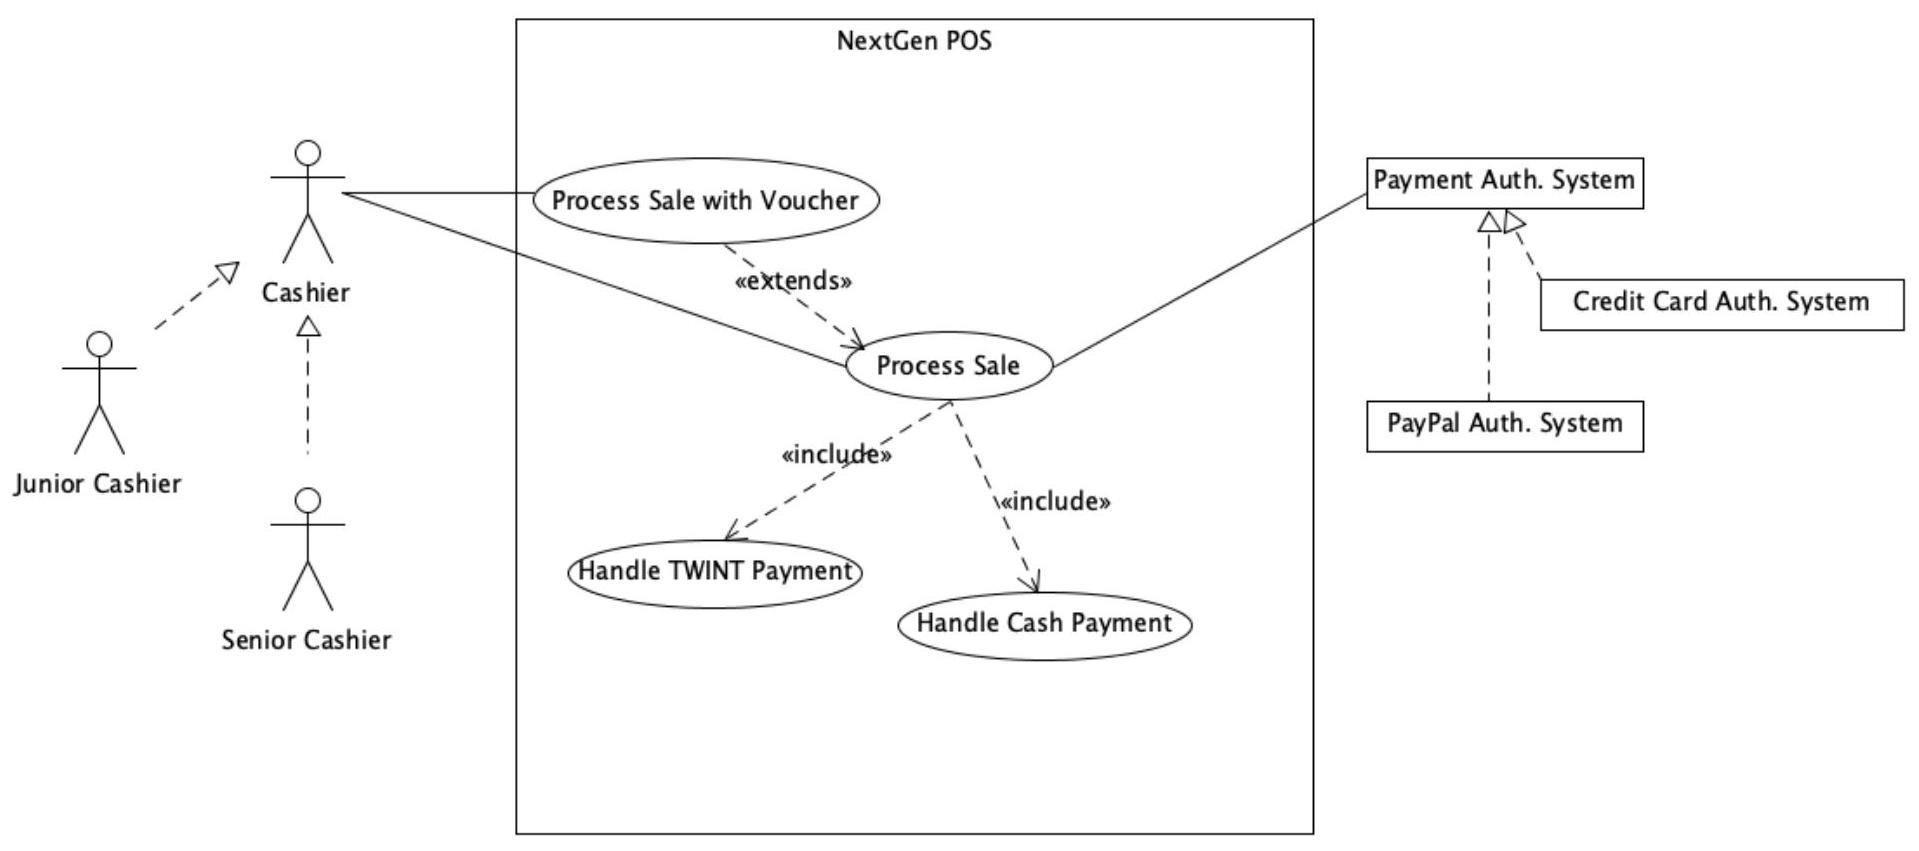
\includegraphics[width=\linewidth]{images/2025_01_02_6d70b14c9f1b57c2938fg-16}
\end{itemize}

\section*{Anwendungsfalldiagramm (Use-Case-Diagramm)}
\begin{itemize}
  \item Zusätzliche Beziehungen im UC-Diagramm
  \item <<extends>>
  \item Eigenständiger UC, der eine Erweiterung eines anderen darstellt, und
  \item ursprünglicher UC nicht verändert werden soll
  \item Sonst besser als Erweiterung im UC-Text einfügen
  \item Akteur-Generalisierung
  \item Um Akteure zusammenzufassen
  \item Kann als „ist-ein"-Beziehung modelliert werden
\end{itemize}

\begin{enumerate}
  \item Wie erfasst man (dynamische) funktionale Anforderungen mit Use Cases
  \item Wie schreibt man gute Use Cases
  \item System-Sequenzdiagramme, Systemoperationen und Verträge
  \item Wie erfasst man zusätzliche funktionale und nicht-funktionale Anforderungen
  \item Wrap-up und Ausblick
\end{enumerate}

\section*{Anwendungsfälle: Brief UC}
\begin{itemize}
  \item Kurze Beschreibung des
\end{itemize}

Anwendungsfalls in einem Paragraphen

\begin{itemize}
  \item Nur Erfolgsszenario
  \item Sollte enthalten
  \item Trigger des UCs
  \item Akteure
  \item Summarischen Ablauf des UCs
  \item Wann?
  \item Zu Beginn der Analyse
  \item Process Sale (brief)
\end{itemize}

Kunde kommt mit seinen Waren zur Kasse. Kassier erfasst alle gekauften Produkte. Am Ende berechnet Kasse den Totalbetrag. Kassier zieht das Geld von Kunden ein und gibt den Betrag in die Kasse ein. Diese berechnet das Rückgeld. Kassier gibt Kunde das berechnete Rückgeld zurück.

\section*{Anwendungsfälle: Casual UC}
\begin{itemize}
  \item Informelle Beschreibung des Anwendungsfalls in mehreren Paragraphen
  \item Erfolgsszenario plus wichtigste Alternativszenarien
  \item Sollte enthalten
  \item Trigger des UCs
  \item Akteure
  \item Interaktion des Akteurs mit System
  \item Wann?
  \item Zu Beginn der Analyse
  \item Process Sale (casual)
  \item Kunde kommt mit seinen Waren zur Kasse. Kassier scannt den Produktcode jedes Produkts ein. Kasse zeigt Artikel und Preis. Kassier korrigiert Menge, falls nötig. Bei Produkten ohne Code gibt der Kassier das Produkt und den Preis, sowie die Menge manuell ein.
  \item Am Ende schliesst Kassier den Einkauf ab. Kasse zeigt den Totalbetrag. Kassier nimmt das Geld vom Kunden entgegen und gibt den bezahlten Betrag in Kasse ein. Kasse berechnet den Retourbetrag und öffnet die Geldschublade. Kassier entnimmt den Retourbetrag und übergibt das Retourgeld dem Kunden. Kassier schliesst Geldschublade und beendet damit den Verkauf.
  \item Kasse druckt die Quittung aus. Kassier übergibt Quittung dem Kunden.
\end{itemize}

\section*{Anwendungsfälle: Fully-dressed UC}
\section*{- Detaillierte Beschreibung des Ablaufs}
 mit allen Alternativszenarien\begin{itemize}
  \item Wann?
  \item Ende der Inception- und v.a. in ElaborationPhase (Anforderungsdisziplin)
  \item Nachdem die meisten UCs identifiziert und kurz beschrieben worden sind
  \item Die wichtigsten UCs (10\%), die die Architektur bestimmen, werden im Detail ausformuliert
  \item Formaler Aufbau
  \item UC-Name
  \item Umfang (Scope)
  \item Ebene (Level)
  \item Primärakteur (Primary Actor)
  \item Stakeholders und Interessen
  \item Vorbedingungen (Preconditions)
  \item Erfolgsgarantie/Nachbedingungen (Success Guarantee)
  \item Standardablauf (Main Sucess Scenario)
  \item Erweiterungen (Extensions)
  \item Spezielle Anforderungen (Special Requirements)
  \item Liste der Technik und Datavariationen (Technology and Data Variations)
  \item Häufigkeit des Auftretens (Frequency of Occurance
  \item Verschiedenes (Miscellaneous)
\end{itemize}

\section*{Anforderungsanalyse: Anwendungsfälle (Use Cases)}
\begin{itemize}
  \item Eigenschaften guter Anwendungsfälle
  \item Aussagekräftiger Titel
  \item Beschreibt Anwenderziel, aktiv formuliert
  \item Beispiel (Akteur Kassier): „Process Sale" (Einen Verkauf abwickeln)
  \item Essentieller Stil (nicht konkreter Stil)
  \item Beschreibt Logik der Interaktion, nicht konkrete Umsetzung
  \item Beispiel (Akteur Kassier):
  \item Konkret: „Kassier tippt die Produkt-ID ein. System zeigt Produktnamen."
  \item Essentiell: „Kassier erfasst das Produkt. System bestätigt Produkt." (z.B. durch Eintippen, Wählen, Scannen, oder per Sprache)
\end{itemize}

\section*{Anforderungsanalyse: Anwendungsfälle (Use Cases)}
\begin{itemize}
  \item Eigenschaften guter Anwendungsfälle
  \item Knappe aber präzise Beschreibung der Interaktion des Standardablaufs
  \item Keine kann-Formulierungen
  \item Alternative Interaktionen sind unter Erweiterungen aufgeführt
  \item Nur Aussensicht (Benutzersicht), keine systeminternen Interaktionen
\end{itemize}

\section*{Anwendungsfälle, und wie weiter?}
\begin{itemize}
  \item Frage
  \item Wie kommen wir von den Anwendungsfällen, die auf abstrakter Ebene die funktionalen Anforderungen an das System beschreiben, zu den konkreten Funktionalitäten, die das System aufweisen muss?
  \item Antwort
  \item Systemsequenzdiagramme
  \item Operation Contracts
\end{itemize}

\begin{enumerate}
  \item Wie erfasst man (dynamische) funktionale Anforderungen mit Use Cases
  \item Wie schreibt man gute Use Cases
  \item System-Sequenzdiagramme, Systemoperationen und Verträge
  \item Wie erfasst man zusätzliche funktionale und nicht-funktionale Anforderungen
  \item Wrap-up und Ausblick
\end{enumerate}

\section*{Systemsequenzdiagramm (SSD)}
School of Engineering nIT Institut für angewandte Informationstechnologie

\begin{itemize}
  \item Ist formal ein UML Sequenzdiagramm
  \item Zeigt Interaktionen der Akteure mit dem System
  \item Welche Input-Events auf das System einwirken
  \item Welche Output-Events das System erzeugt
  \item Ziel
  \item Wichtigste Systemoperationen identifizieren, die das System zur Verfügung stellen muss (API) für einen gegebenen Anwendungsfall\\
system as black box\\
the name could be "NextGenPOS" but "System" keeps it simple\\
the ":" and underline imply an instance, and are explained in a later chapter on sequence diagram notation in the UML\\
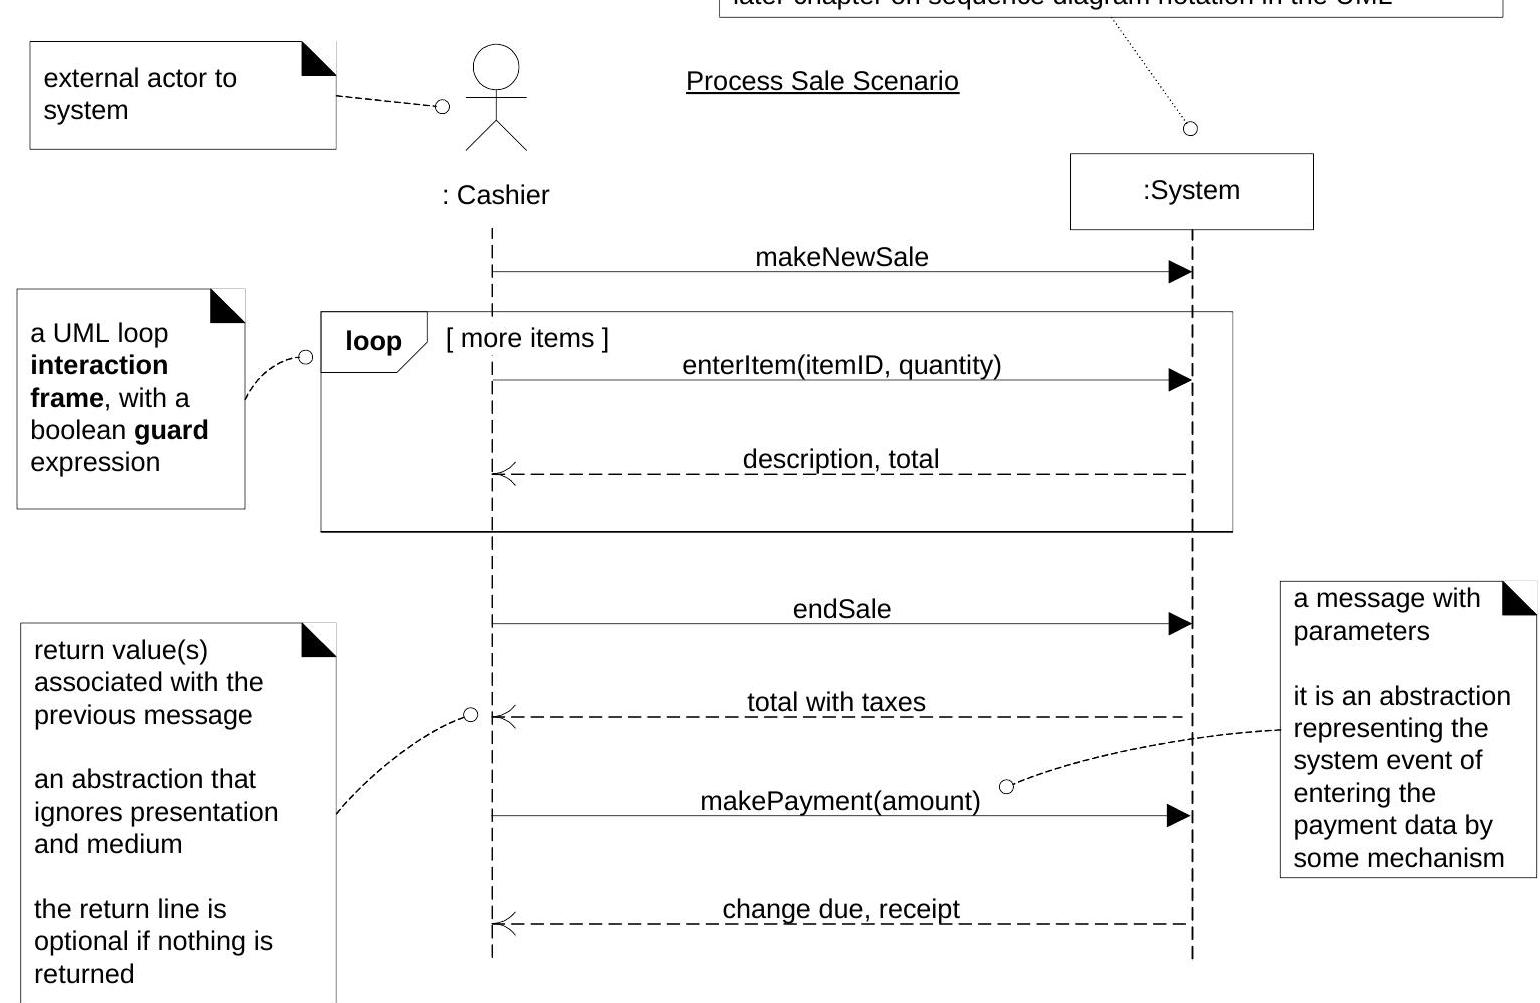
\includegraphics[width=\linewidth]{images/2025_01_02_6d70b14c9f1b57c2938fg-26}
\end{itemize}

\section*{Systemoperation}
School of Engineering

\begin{itemize}
  \item Formal wie ein Methodenaufruf
  \item Treffender Name, der die Absicht des Akteurs repräsentiert
  \item Evtl. mit Parametern
  \item Information, die für die Ausführung der Systemoperation nötig sind, aber noch nicht im System vorhanden sind
  \item Details zu den Parametern sollten im Glossar erläutert werden
  \item Durchgezogener Pfeil für Methodenaufruf
  \item Rückgabewert
  \item Kann fehlen, falls unwichtig
  \item Kein Methodenaufruf, sondern indirektes Update des UI (deshalb gestrichelte Linie)\\
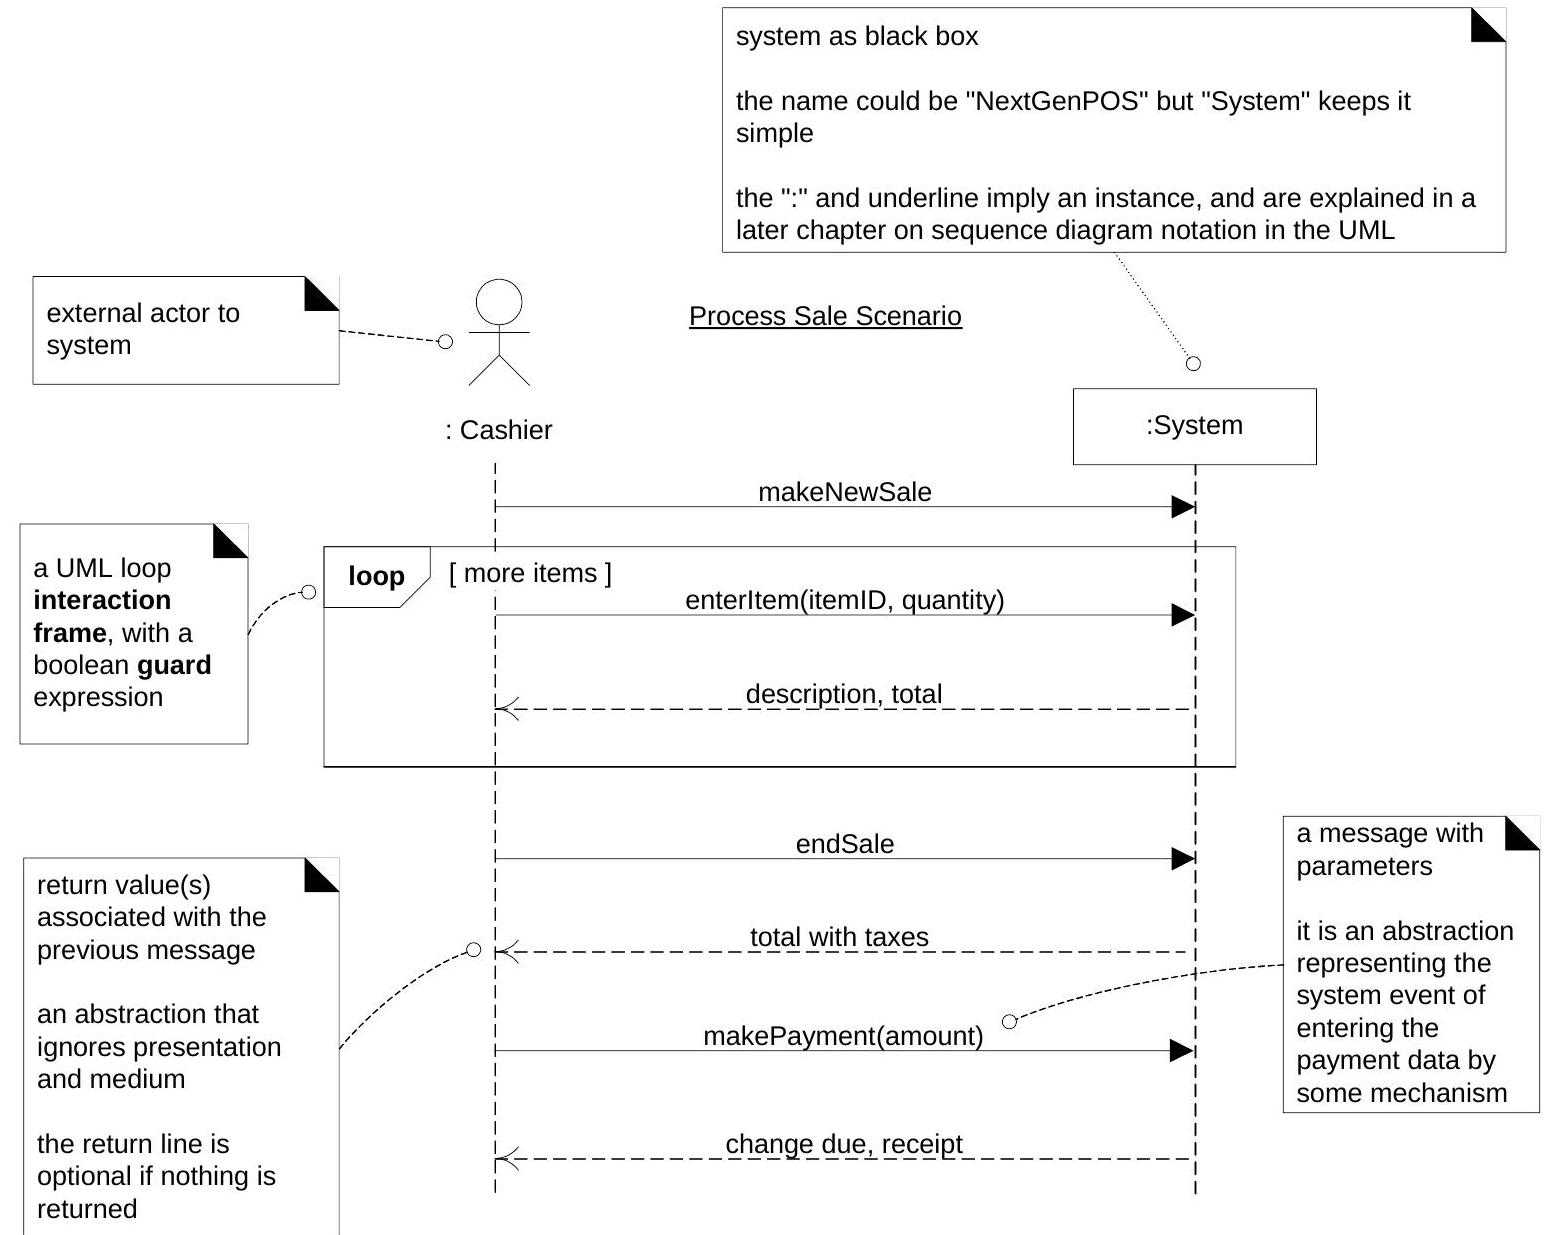
\includegraphics[width=\linewidth]{images/2025_01_02_6d70b14c9f1b57c2938fg-27}
\end{itemize}

\section*{SSD für Interaktionen zwischen Systemen}
\begin{itemize}
  \item SSD können auch Interaktionen zwischen SuD und externen unterstützenden System zeigen\\
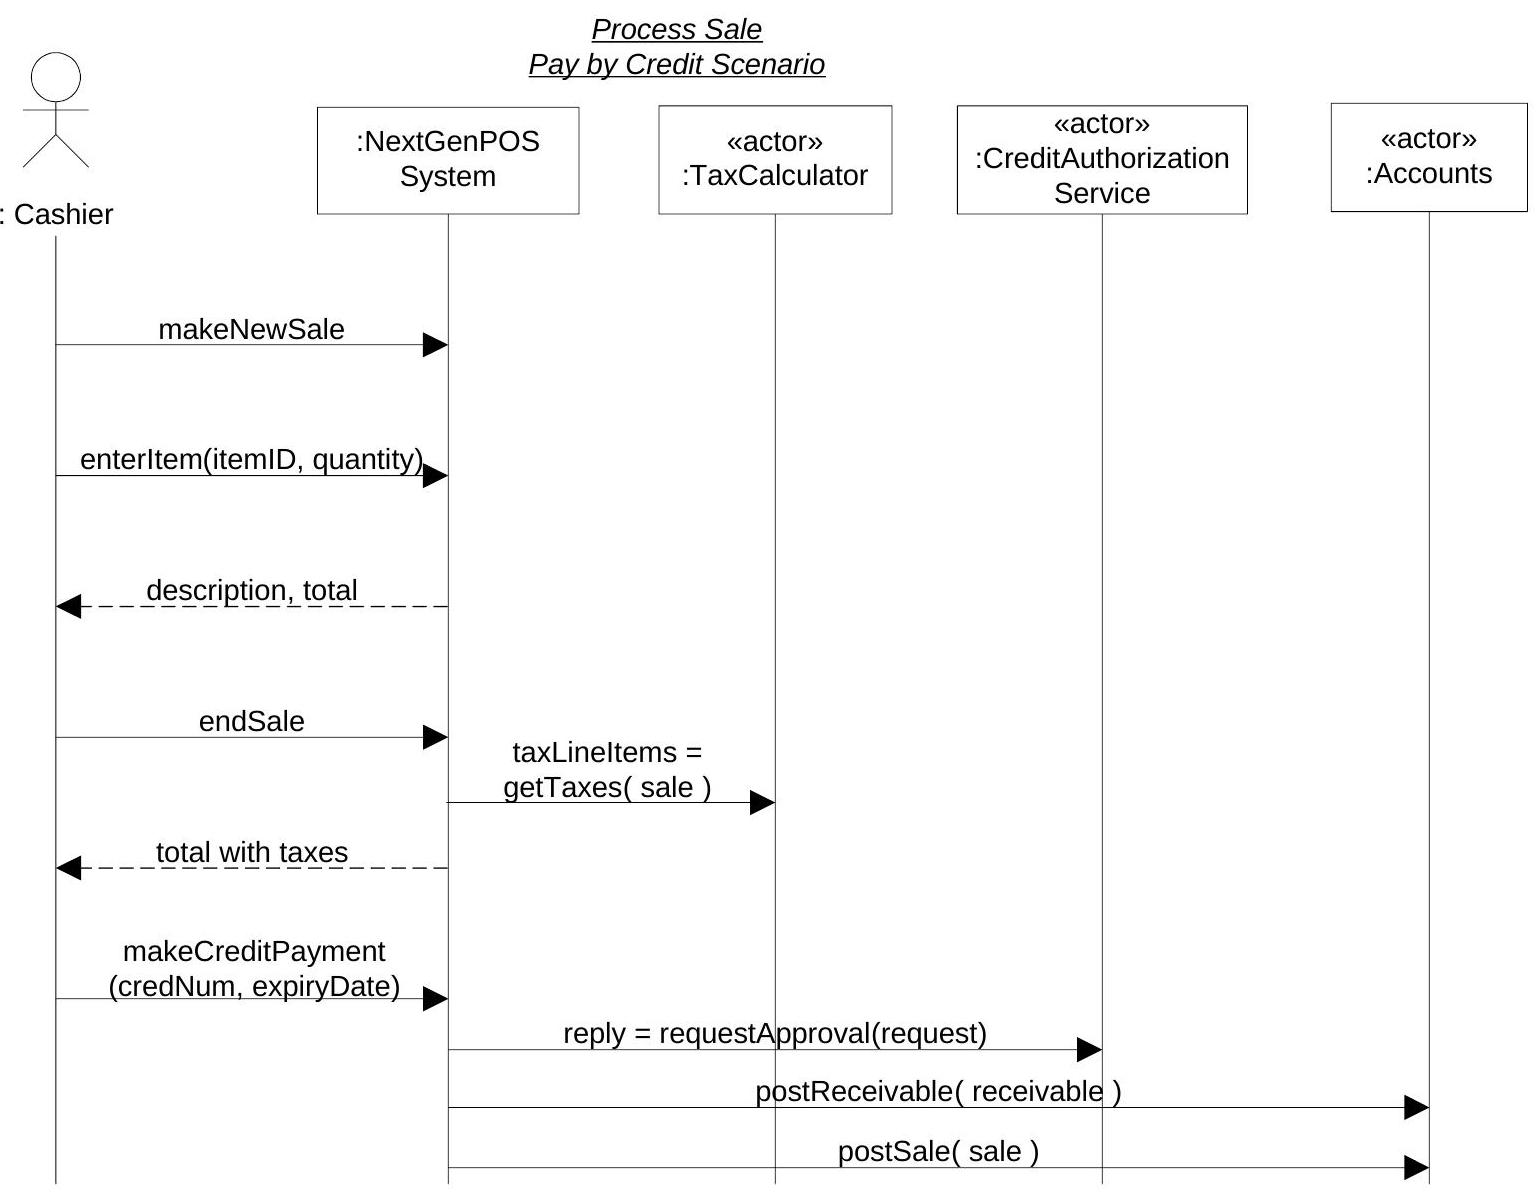
\includegraphics[width=\linewidth]{images/2025_01_02_6d70b14c9f1b57c2938fg-28}
\end{itemize}

\section*{Operation Contract}
\begin{itemize}
  \item Eine (System) Operation kann mit einem Vertrag noch genauer spezifiziert werden
  \item Name plus Parameterliste
  \item Vorbedingung
  \item Was muss zwingend erfüllt sein, damit Systemoperation aufgerufen werden kann
  \item Nachbedingung
  \item Was hat sich alles geändert im System nach Ausführung der Systemoperation
  \item Erstellte/gelöschte Instanzen, Assoziationen
  \item Geänderte Attribute
  \item Basiert auf Domänenmodell
\end{itemize}

\section*{Contract CO2: enterltem}
\begin{itemize}
  \item Operation:
\end{itemize}

\begin{verbatim}
enterItem(idemID: ItemID,
quantity: integer)
\end{verbatim}

\begin{itemize}
  \item Querverweis: UC Process Sale
  \item Vorbedingungen:
  \item Verkauf muss gestartet sein
\end{itemize}

Zeitform beachten!

\begin{itemize}
  \item Nachbedingungen
  \item SaleLineItem-Instanz sli (ist) erstellt
  \item sli mit aktueller Sale-Instanz verknüpft
  \item sli.quantity auf quantity gesetzt
  \item sli mit entsprechender ProductDescription verknüpft (gemäss itemID)
\end{itemize}

\section*{Operation Contract}
\begin{itemize}
  \item Wann Operation Contracts?
  \item Nur wenn aus einem Anwendungsfall nicht klar wird, was die Systemoperation genau machen muss
  \item Meist nur bei sehr komplizierten Operationen und/oder
  \item Wenn Entwicklung der Systemoperation ausgelagert wird (anderes Team, externe Entwickler)
  \item Erst gegen Ende des Meilensteins Lösungsarchitektur oder kurz vor Start des Designs der Systemoperation
\end{itemize}

\section*{Nutzen von SSD und Systemoperationen}
\begin{itemize}
  \item Systemoperationen definieren die Schnittstelle (API) des Systems
  \item Während dem Design
  \item wird das System ausgehend von den Systemoperationen entwickelt (anhand der Verträge)
  \item Das UI-Team kann parallel das UI entwickeln unter Verwendung der vereinbarten Systemoperationen (und ihren Verträgen)
  \item SSD können auch zur Darstellung der Kommunikation von Subsystemen verwendet werden (z.B. bei Client-Server-Architektur)
  \item Achtung Frameworks!
  \item UI- und andere Frameworks geben häufig gewisse Systemoperationen vor, die das System implementieren muss
  \item Sollte man bei den SSD bereits berücksichtigen
\end{itemize}

\begin{enumerate}
  \item Wie erfasst man (dynamische) funktionale Anforderungen mit Use Cases
  \item Wie schreibt man gute Use Cases
  \item System-Sequenzdiagramme, Systemoperationen und Verträge
  \item Wie erfasst man zusätzliche funktionale und nicht-funktionale Anforderungen
  \item Wrap up und Ausblick
\end{enumerate}

\section*{Weitere Anforderungen}
\begin{itemize}
  \item Die UCs beschreiben einen grossen Teil der funktionalen Anforderungen aus Benutzersicht
  \item Es gibt aber weitere funktionale und nicht-funktionale Anforderungen (Qualitätsanforderungen und Randbedingungen), die schlecht in UCs beschrieben werden können
  \item Diese werden als zusätzliche Anforderungsspezifikation formuliert (Supplementary Specification)
  \item Zusätzliche Anforderungen
  \item Können als Anforderungsstatement oder als User-Story (agile SWE) formuliert werden
  \item Bsp:
  \item Anforderungsstatement:\\
„Das Kassensystem muss in weniger als 1 Minute aufgestartet sein"
  \item User-Story:
\end{itemize}

Als Kassier möchte ich, dass bei mehreren gleichen Artikeln der Einzelpreis, die Anzahl und der Gesamtpreis angezeigt werden, damit ich einen schnellen Überblick habe.

\section*{Weitere Anforderungen}
\begin{itemize}
  \item Anforderungsstatements
  \item Sollten als Anforderung formuliert werden
  \item Das System muss/soll mindestens/darf nicht...
  \item Sollten messbar/verifizierbar sein
  \item Sie müssen dem Auftraggeber irgendwann belegen, dass ihr System diese Anforderung erfüllt
  \item So wenig wie nötig
  \item Nur Anforderungen stellen, die auch wirklich von jemandem begründet gefordert werden
  \item Keine ersten Lösungsideen als Forderungen formulieren
  \item „Das System muss eine Web-App sein"
\end{itemize}

\section*{- User-Stories}
\begin{itemize}
  \item Sagen in einem Satz wer, was, warum fordert
  \item Erfüllen damit einige der Bedingungen automatisch
  \item Die anderen sollten aber auch bei UserStories erfüllt sein
  \item Messbarkeit/Verifizierbarkeit (z.B. durch Akzeptanzkriterien)
\end{itemize}

\section*{Weitere Anforderungen: FURPS+}
\section*{- Checkliste für zusätzliche Anforderungen}
\begin{itemize}
  \item Functionality (Funktionalität)
  \item Features, Fähigkeiten, Sicherheit
  \item Usability (Gebrauchstauglichkeit)
  \item Siehe Usability-Anforderungen (LE02)
  \item Accessibility (Benutzer mit spez. Bedürfnissen)
  \item Reliability (Zuverlässigkeit)
  \item Fehlerrate, Wiederanlauffähigkeit, Vorhersagbarkeit, Datensicherung
  \item Performance (Performanz)
  \item Reaktionszeiten, Durchsatz, Genauigkeit, Verfügbarkeit, Ressourceneinsatz
  \item Supportability (Unterstützbarkeit)
  \item Anpassungsfähigkeit, Wartbarkeit, Internationalisierung, Konfigurierbarkeit
  \item Implementation
  \item HW, Betriebssysteme, Sprachen, Tests, Werkzeuge,..
  \item Interface
  \item Schnittstellen von ext. Systemen, Protokolle
  \item Operations
  \item Betriebliche Aspekte
  \item Packaging (Verpackung)
  \item Auslieferung physisch, logisch (Container, Plugin,..)
  \item Legal
  \item Lizenzen, rechtl. Rahmenbedingungen
\end{itemize}

\section*{Glossar}
\begin{itemize}
  \item Einfaches Glossar
  \item Definiert die Begriffe, die in diesem Projekt und im SW-Produkt verwendet werden
  \item Kann beliebige Elemente enthalten
  \item Wichtige Begriffe, Konzepte des Domänenmodells, Attribute, Parameter von Operationen
  \item Data Dictionary
  \item Definiert zusätzlich Datenformate, Wertebereiche, Validierungsregeln
  \item Empfehlungen Glossar
  \item So früh wie möglich mit Glossar beginnen, sobald der erste Begriff auftaucht, der nicht sofort allen klar ist
  \item Fortwährend aufdatieren, sobald weitere Begriffe, Konzepte etc. auftauchen, die nicht allen sofort klar sind
  \item In der Kommunikation untereinander, die Begriffe des Glossars verwenden
  \item Fördert Klarheit in der Kommunikation unter den Projektmitgliedern
  \item Für dieselbe Sache nur einen Begriff verwenden (wenn möglich)
\end{itemize}

\begin{enumerate}
  \item Wie erfasst man (dynamische) funktionale Anforderungen mit Use Cases
  \item Wie schreibt man gute Use Cases
  \item System-Sequenzdiagramme, Systemoperationen und Verträge
  \item Wie erfasst man zusätzliche funktionale und nicht-funktionale Anforderungen
  \item Wrap-up und Ausblick
\end{enumerate}

\begin{itemize}
  \item Ausgehend von den Kontextszenarien werden die funktionalen Anforderungen immer mehr konkretisiert.
  \item Anwendungsfälle (Use Cases)
  \item Beschreiben die konkrete Interaktion der Akteure mit dem System (lösungsneutral)
  \item Systemsequenzdiagramme (System Sequence Diagram)
  \item Identifizieren die notwendigen Systemoperationen, die das System für die Anwendungsfälle zur Verfügung stellen muss
  \item Systemoperationen und Verträge (Operation Contracts)
  \item Spezifizieren die Systemoperationen im Detail
\end{itemize}

\section*{Ausblick}
\begin{itemize}
  \item In dieser Lerneinheit haben Sie gelernt, wie Sie «dynamische» funktionale Anforderungen aus den Interaktionsbedürfnissen der Benutzer ableiten können.
  \item In der nächsten Lerneinheit werden Sie lernen,
  \item wie Sie die Problemdomäne an sich im Detail verstehen und kommunizieren können.
\end{itemize}

\section*{Quellenverzeichnis}
[1] M. Richter and M. D. Flückiger, Usability und UX kompakt: Produkte für Menschen, 4th ed. Springer Vieweg, 2016.\\[0pt]
[2] Larman, C.: UML 2 und Patterns angewendet, mitp Professional, 2005\\[0pt]
[3] Seidel, M. et al.: UML @ Classroom: Eine Einführung in die objektorientierte Modellierung, dpunkt.verlag, 2012\\[0pt]
[4] Martin, R. C.: Clean Architecture: A Craftsman's Guide to Software Structure and Design, mitp Professional, 2018


\end{document}